%  Explain your design methodology, such as your design steps, lab work
%  partitioning, special techniques used, etc. Clearly explain any
%  special programming considerations (e.g., explain how and why you set
%  up control registers, how and why you check for flags, etc.)

\section{Design Solution}
The design solution involved dividing the project into parts, including
planning and implementation divisions which were then separated further
to allow even distribution of the work. Information and reference was
primarily found through the reference manuals for both the \gls{stm} and
project board \cite{ref,board}.
\subsection{Planning}
Before beginning the implementation phase, planning was done to
determine who would primarily focus on which parts of the project, and
come up with some broad design ideas.
\subsubsection{Work Partitioning}
Based on experience from the first lab, and personal preference, lab
work was partitioned accordingly. The project was split into the
embedded programming and accessory circuit design/implementation, where
the majority of the embedded programming was assigned to Tayler Mulligan
and the accessory timer circuit to Raymond Bamford. The partitioning was
not strict, with members collaborating where necessary or convenient.

\subsubsection{Technique and Technologies}
Git and GithHub were utilized for the project to provide team access and
syncing between lab computers (see
\url{https://github.com/tamul/ceng355-lab-project}). The source code was
split into three files: \filename{main.c} (see \ref{app:main}), containing the main program;
\filename{analog.c} (see \ref{app:analog}), containing \gls{adc},
\gls{dac}, and frequency monitoring
code; and \filename{lcd.c} (see \ref{app:lcd}), containing code related
to the \gls{lcd}; each with corresponding header files. Each file
provided initialization functions for the components and abstracted
functions to control the components, such as:

\begin{lstlisting}[numbers=none]
void spi_init(void),
void lcd_cmd(uint8_t data),
void lcd_char(char c),
\end{lstlisting}

etc. in \lstinline{lcd.h}; and:

\begin{lstlisting}[numbers=none]
void dac_init(void),
void adc_init(void)
uint16_t adc_read(void),
void dac_write(uint16_t),
\end{lstlisting}

etc. in \lstinline{analog.h}. See the attached listings in the
appendices for complete definitions and declarations.

\subsection{Software Implementation}
The main program called functions provided by \lstinline{analog.h} and
\lstinline{lcd.h} to sequentially initialize each component. Components
were initialized in the order of: the \gls{adc}, the \gls{dac}, the
\gls{lcd}, and the frequency monitor. Details of registers and other
technical notes are available in the reference manual published by
STMicroelectronic's \cite{ref}.

\lst{Initialization order}{code:init-order}{42}{57}{src/main.c}

\subsubsection{ADC Initialization}
Initialization of the gls{adc} requires initialization of the \gls{gpio}
port C interface (to control the POT\_EN signal of the Project Board),
GPIOC (to read the potentiometer value), and the gls{adc}. The C code in
Listing~\ref{code:adc-gpioc-conf} comprises the initialization of the
GPIOC register for the gls{adc}.

\lst{GPIO configuration for ADC}{code:adc-gpioc-conf}{35}{48}{src/analog.c}

Firstly, the GPIOC clock is ensured to be running, followed by
configuration of the pins. The pins are put in a push-pull output
configuration at the highest speed, without any pull-up or pull-down
resistors.

\lst{ADC configuration}{code:adc-conf}{50}{74}{src/analog.c}

Next the \gls{adc} proper is initialized: the C code in
Listing~\ref{code:adc-conf} accomplishes this.  The \gls{hsi} clock, which
supplies the \gls{adc}'s clock, is enabled and the \gls{adc} started in preparation
for configuration. Lines~57-68 configure the gls{adc}: setting the clock as
the dedicated (\gls{hsi}) clock, selecting input channel 0 (corresponding to
parallel pin A0), continuous conversion mode is enabled to continuously
provide the digitized value of the PA0 pin. Finally, the function
triggers conversion to start after waiting until the gls{adc} reports that it
has stabilized.

\subsubsection{DAC Initialization}
Enabling the \gls{dac} requires configuration of the PA4 pin and
initialization of the \gls{dac} clock. Listing~\ref{code:dac-init} shows
the C code initializing the \gls{dac}.

\lst{DAC configuration}{code:dac-init}{78}{92}{src/analog.c}

The mode of PA4 is set to an open-drain analog output, allowing a
variable voltage to be placed on PA4, with pull-up and pull-down
pins disabled, at the highest speed setting to ensure the pin updates
quickly. Next, the \gls{dac}'s clock is enabled and the \gls{dac}
enabled by writing the \gls{dac}'s \gls{cr}'s enable bit.

\subsubsection{LCD Initialization}

To initialize the \gls{lcd}, the \gls{spi}, GPIOB, and GPIOC clocks are
all initialized (Listing~\ref{code:lcd-init-clocks}).

\lst{SPI, GPIOB, GPIOC clock enable}{code:lcd-init-clocks}{15}{21}{src/lcd.c}

The \gls{lck} pin (PC2) of the \gls{spi} shift-register is set to output
mode, and the \gls{mosi} (PB5) and \gls{sck} (PB3) \gls{spi} pins are
set to alternate function mode (Listing~\ref{code:lcd-init-output}).

\lst{SPI pin mode configuration}{code:lcd-init-output}{23}{30}{src/lcd.c}

Each \gls{spi} related pin is set to push-pull mode with pull-up and
pull-down resistors disabled and high-speed mode
(Listing~\ref{code:lcd-init-output-conf}).

\lst{SPI pin output configuration}{code:lcd-init-output-conf}{32}{45}{src/lcd.c}

After configuring the output pins, \gls{tim3} is configured, allowing
\gls{spi} writes to be delayed and the \gls{lcd} time to complete
the commands sent:

\lst{TIM3 configuration}{code:lcd-tim3-conf}{47}{62}{src/lcd.c}

The clock for \gls{tim3} is enabled, then the clock is configured to use
buffered auto-reload, count down from the set \lstinline{CNT} register
value, stop in the event of an overflow (which should never occur), and
only interrupt in the event of an overflow not when the counter reaches
0. This configuration allows a value to be written to the timer which
then counts down to 0, and the timer can be polled until the count is
low enough (and enough time has passed), then allowing another command to be
sent. This avoids the potential for an overflow if the counter was
initialized to zero and counted up to or past the desired value. \\

The prescaler is set to 0, the auto-reload delay set to the lowest
possible, writing to the \lstinline{EGR} register is a carry-over from
other timer initializations and is not necessary in this case; then, the
\lstinline{MAX\_DELAY} value (the maximum time the LCD will take to
execute a command) is loaded into the timer's \lstinline{CNT}
register, and the timer finally started. This timer is utilized
by checking the \lstinline{CNT} value rather than the updates generated
for the purpose of allowing a potentially shorter delay. In the end this
potential for a shorter delay was not utilized, however checking the
\lstinline{CNT} register rather than an update bit was retained.

Next, in Listing~\ref{code:spi-init}, \gls{spi} is configured and
enabled with: unidirectional transmit, master mode, a data-size of 8
bits, \gls{cpol} and \gls{cpha} are set for a falling edge clock pulse, software chip select, a 256 baud-rate
prescaler, \gls{msb} first output, and a 7 bit \gls{crc} polynomial.

\lst{SPI initialization}{code:spi-init}{64}{78}{src/lcd.c}

Finally, in Listing~\ref{code:lcd-init}, the command interface and
the display of the \gls{lcd} are initialized: the \gls{lcd} is set to a
4-bit interface with 2 lines, followed by the LCD being cleared and
homed with display shift disabled and cursor movement direction set to
the right, cursor blinking being disabled. The persistent, unchanging
characters of the \gls{ui} are then written to the \gls{lcd}.

\lst{LCD initialization}{code:lcd-init}{80}{114}{src/lcd.c}

\subsubsection{Frequency Monitor Initialization}

Initialization of the frequency monitor required the GPIOA and
\gls{tim2} clocks to be enabled, GPIOA pin 1 configured as an input,
and configuration of \gls{tim2}. \\

PA1 is first configured with the C code in Listing~\ref{code:fm-init-gpio}.

\lst{GPIOA pin 1 configuration}{code:fm-init-gpio}{94}{100}{src/analog.c}

The GPIOA clock is first ensured to be enabled, followed by the setting
pin PA1 to input mode with pull-up and pull-down resistors disabled.
\gls{tim2} is then initialized, seen in Listing~\ref{code:fm-init-tim2}.

\lst{TIM2 initialization}{code:fm-init-tim2}{102}{115}{src/analog.c}

\gls{tim2} is configured with a buffered auto-reload in count up mode,
with stop on overflow set and updates events enabled with interrupts
only enabled for overflow. This allows the timer to notify in the event
of an iInterrupt and avoid erroneous frequencies measurements when the
frequency drops below a corresponding period of approximately
\SI{90}{s}. \\

Next, the interrupt routines are configured through the \gls{nvic} as
seen in Listing~\ref{code:fm-init-nvic}.

\lst{NVIC configuration}{code:fm-init-nvic}{117}{137}{src/analog.c}

The priority of the interrupt is set to 0, as it is one of only two
interrupts that should be firing in this system. \gls{tim2} interrupts
are enabled in the \gls{nvic} to allow notifiication of overflow, and
interrupt generation is enabled in \gls{tim2}. The external interrupt
line carrying the external waveform, \gls{exti1}, is mapped to PA1. The
external interrupt line has interrupts enabled with a rising-edge
trigger and interrupts for \gls{exti1} unmasked in the \gls{nvic} so
they are processed. Finally, \gls{exti1} is configured to have a
priority  of 0 in the \gls{nvic}, and enabled.

\subsubsection{LCD Implementation} \label{sec:lcd-imp}
Utilization of the LCD was accomplished through the
\lstinline{void lcd_char(char c)} and
\lstinline{void lcd_cmd(uint8_t data)} functions. \lstinline{lcd_char}
provides an interface to specify a character which is then translated to
the proper LCD command and displayed at the current cursor position.
\lstinline{lcd_cmd} does not translate it's input, instead implementing
the transmission of 8 bits of data to the LCD over the 4 bit interface.
Definitions of \lstinline{lcd_char} and \lstinline{lcd_cmd} can be seen
in Listing~\ref{code:lcd-functions}

\lst{LCD interface function definitions}{code:lcd-functions}{116}{163}{src/lcd.c}

Both commands split the 8 bits of data to be sent into 4 bit packets to
be sent over the 4 bit interface: where 4 bits of the data sent are
control bits and 4 bits are data. The difference between the two
commands resides in the control bits, where \lstinline{lcd_char} has the
\gls{rs} bit LOW whereas \lstinline{lcd_cmd} send a HIGH \gls{rs} bit.
\\

Both functions utilize \lstinline{void spi_write(uint8_t data)}, a
function providing an abstracted interface to utilize the 74HC164
serial-in, parallel-out shift register which interfaces with the
\gls{lcd}. The command ensures suitable time has passed by polling
\gls{tim3}, where it then sets the \gls{lck} signal LOW, loads the data
into the shift register over \gls{spi} before finally setting the
\gls{lck} pin HIGH again and resets the \gls{tim3} delay counter.

Displaying frequency and resistance information on the \gls{lcd} is
accomplished by first setting up the \gls{ui} by writing the persistent
characters, where the underscores between represent spaces which are
updated with the read values:

\begin{lstlisting}
	F:____Hz
	R:____Oh
\end{lstlisting}

When the frequency monitor reads an updated value (see~\ref{sec:fm-imp}
for details) the LCD is updated with the new resistance and calculated
frequency values. When these values are received, the code in
Listing~\ref{code:lcd-value-update} updates the frequency of the \gls{ui}.

\lst{LCD value update}{code:lcd-value-update}{169}{174}{src/analog.c}

The value of the frequency is converted to an array of ASCII characters
by calling \lstinline{char* num_to_ascii(uint16_t)}
(Listing~\ref{code:num-to-ascii}) , which are then written to the LCD.
The loop decrements to read the array from end to start, as the way
\lstinline{num_to_ascii} operates stores the digits least significant
digit first. The same method is used to update the resistance value,
however the resistance value is rounded to the nearest 100 as the
frequency does not change until the resistance varies by approximately
this amount, and to improve readability by reducing flickering of the
digits.

\lst{Convert a value to ASCII characters}{code:num-to-ascii}{165}{184}{src/lcd.c}


\subsubsection{Frequency Monitor Implementation} \label{sec:fm-imp}

The frequency monitor's main components consist of \gls{tim2} and an
interrupt routine triggered by \gls{exti1}. Defined in
Listing~\ref{code:fm-imp}, \lstinline{void EXTI0_1_IRQHandler()} is the
routine called when the input PA1 sees a rising-edge.

\lst{Frequency monitor interrupt routines}{code:fm-imp}{139}{198}{src/analog.c}

Every $2n, n=0,1,\dots$  executions (executions 0,2,\dots where
\lstinline{first_edge=1}) of this routine:

\begin{enumerate}
	\item Interrupts are disabled.
	\item The interrupt request flag is checked.
	\item The count of \gls{tim2} to 0 and the timer started
	\item The interrupt flag is cleared and interrupts are re-enabled.
	\item The service routine returns.
\end{enumerate}

Every $2n+1, n=0,1,\dots$ executions (executions 1,3,\dots where
\lstinline{first_edge=0}) of this routine:

\begin{enumerate}
	\item Interrupts are disabled.
	\item The interrupt request flag is checked.
	\item The \gls{tim2} clock is stopped.
	\item The current count is stored in \lstinline{uint32_t count}.
	\item The frequency and resistance displayed on the \gls{lcd} is
		updated (see~\ref{sec:lcd-imp}).
	\item \gls{tim3} is utilized to delay updates to a reasonable period
		(to reduce flickering of the numbers on the \gls{lcd}).
	\item The interrupt flag is cleared and interrupts are re-enabled.
	\item The service routine returns.
\end{enumerate}

The end result is measurement of the time between 2 successive
rising-edges, giving the frequency of the input waveform. \\ 

The \lstinline{void TIM2_IRQHandler()} interrupt routine, also visible in
Listing~\ref{code:fm-imp}, is the routine called in the event of an
interrupt generated by the \gls{tim2}, which only occurs in the event of
an overflow.



\subsection{Hardware Implementation}
\begin{figure}
	\caption{555 Timer Configuration \cite{slide:interface}}
	\centering
	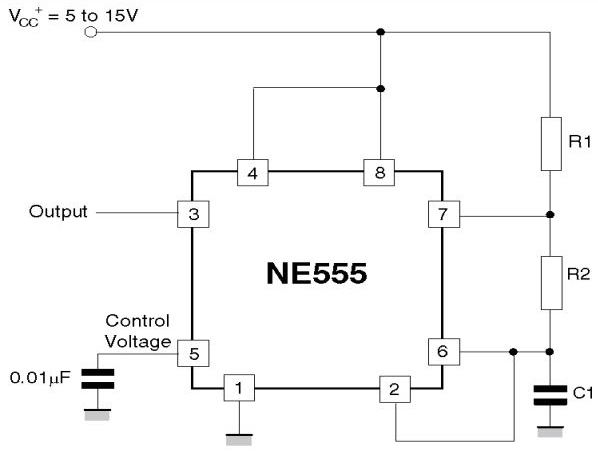
\includegraphics[width=\textwidth]{555-timer}
	\label{fig:555}
\end{figure}


\subsection{Test Procedures}
Tests of the system were conducted in a unit manner: each individual
component was tested before testing components together.

\subsubsection{External PWM Signal Generator}
The \gls{pwm} generator was tested by building up the circuit and
providing a variable voltage through a signal generator's DC supply
function, and the output measured with the oscilloscope to ensure
varying the voltage resulted in a changing frequency.

\subsubsection{Potentiometer and ADC System}
The \gls{adc} and potentiometer was tested by supplying the
potentiometer to the analog input pin PA1 and printing the digitized
analog value to the trace of the \gls{stm}.

\subsubsection{DAC System}
The \gls{dac} system was tested using the \gls{adc} by writing the value
measured by the \gls{adc} to the \gls{dac}'s output register and
measuring the outputted voltage and ensuring it varied with varying
the resistance of the potentiometer.

\subsubsection{LCD System}
Testing the \gls{lcd} was conducted with the other components working,
where the test was simply getting the desired message to print.
Initially that desired message was any symbol appearing on the display;
and after debugging, the frequency and resistance value display.

\subsubsection{Complete System}
To test the complete system, the external 555 timer-based \gls{pwm} signal
generator output was connected to both the \gls{stm} board and oscilloscope
such that the frequencies could be compared. The potentiometer was
varied and the generated \gls{pwm} signal's frequency was measured on
both the oscilloscope and the \gls{stm} board as displayed on the
\gls{lcd}: they were found to coincide. Resistance measurement was
confirmed by linearly varying the potentiometer between either extreme
and ensuring the resistance displayed on the \gls{lcd} linearly varies
between \SI{0}{\ohm} and \SI{5}{\kilo\ohm}.


\subsection{Test Results} The results of testing with the above
specified procedures including range, resolution, and measurement error
were recorded.

\subsubsection{Resistance Measurement}
The measured resistance range was the full range provided by the
potentiometer (\SI{0}{\ohm}). As the range of values available from the
\gls{dac} was that provided by a 12-bit integer (0 to 4095) and the
resistance of the potentiometer varied between 0 and 5000, the
measurement resolution of the potentiometer was slightly over
\SI{1}{\ohm}, $\frac{5000}{4095}\approx1.221$\si{\ohm}. The error in
measurement was less than could be measured with the test setup.

\subsubsection{Frequency Production and Measurement}
The frequency of the resulting \gls{pwm} signal varied between
281-535\si{\hertz} in increments of around \SI{20}{\hertz}, or steps of
approximately \SI{400}{\ohm} of change in the potentiometer. The coarse
resolution was caused The measurement error of the frequency in the
available range was less than \SI{1}{\hertz}.

\subsubsection{Limitations}
The largest limitation of the system was the range of frequency the
design external PWM circuit was capable of producing with the available
voltage range from the \gls{stm} board's analog output pin. Additional
limitations came from the \gls{lcd} display. With the \gls{lcd}'s size
of 8x2 only 4 digit values could be displayed. The severe of
ghosting of the \gls{lcd} also limited the viable update speed: when the
display was updated too quickly the two least significant digits, which
changed the most, tended to blend together and become undecipherable;
this was solved by eliminating the two least significant digits as there
value did not tend to influence the produced frequency, which relied
more on the two most significant digits.
